\documentclass[a4paper, 12pt]{article}

% Русский язык
\usepackage[T2A]{fontenc}
\usepackage[utf8]{inputenc}
\usepackage[english,russian]{babel}

% Картинки
\usepackage{graphicx}
\graphicspath{{images/}}
\DeclareGraphicsExtensions{.pdf,.png,.jpg}
\usepackage{wrapfig}

% Математика
\usepackage{amsmath,amsfonts,amssymb,amsthm,mathtools} 

% Параметры страницы
\usepackage[left=2cm,right=2cm,top=2cm,bottom=3cm,bindingoffset=0cm]{geometry}

\usepackage{enumitem,xparse}
\usepackage{caption}
\usepackage{subcaption}
\usepackage{float}

\usepackage{hyperref}

\begin{document}

\newgeometry{left=2cm,right=2cm,top=2cm,bottom=1cm,bindingoffset=0cm}

\begin{titlepage}
    \begin{center}

        \vspace*{5cm}

        {\Huge Московский Физико-Технический Институт}\\[2cm]

        {\LARGE Лабораторная работа №3.2.6}\\[0.25cm]

        \noindent\rule{\textwidth}{1pt}
        \vspace*{-0.25cm}

        {\huge \textbf{Изучение гальванометра}}

        \noindent\rule{\textwidth}{1pt}

        \vfill

    \end{center}

    \begin{flushright}
        \begin{minipage}{0.45\textwidth}
            {\Large
                Выполнил:\\
                Студент 2 курса ФАКТ\\
                Группа Б03-502\\
                Подмосковнов Лев
            }
        \end{minipage}
    \end{flushright}

    \vfill

    \begin{center}
        Долгопрудный\\2026
    \end{center}

\end{titlepage}
\restoregeometry

\setcounter{page}{2}

\section{Цель работы}
Изучение работы высокочувствительного зеркального гальванометра магнитоэлектрической системы в режимах измерения постоянного тока и электрического заряда.

\section{В работе используются:}
\begin{itemize}
    \item зеркальный гальванометр с осветителем и шкалой
    \item источник постоянного напряжения
    \item делитель напряжения
    \item магазин сопротивлений
    \item эталонный конденсатор
    \item вольтметр
    \item переключатель
    \item ключи
    \item линейка
\end{itemize}

\section{Теоретические положения}

\textit{Баллистический гальванометр} -- электроизмерительный прибор магнитоэлектрической системы, отличающийся высокой чувствительностью к току и сравнительно большим периодом свободных колебаний. \par
На помещённую в магнитное поле обтекаемую током рамку гальванометра действуют момент закрученной нити, момент магнитных сил и тормозящий момент (зависит от сил сопротивления воздуха и от вихревых токов). Учитывая все эти моменты, уравнение движения рамки принимает вид
\begin{center}
    $\ddot \varphi + 2 \gamma \dot \varphi + \omega_0^2\varphi = KI $,
\end{center}
где $\gamma$ -- коэффициент затухания подвижной системы гальванометра, $\omega_0$ -- собственная частота колебаний рамки

Динамическая постоянная гальванометра определяется при пропускании через рамку постоянного тока:
\begin{center}
    $C_I = \frac{I}{\varphi} = \frac{D}{BSN}$,
\end{center}
где $B$ - индукция магнитного поля в рамке, $S$ - площадь одного витка рамки, $D$ - модуль кручения нити. \par
При пропускании коротких импульсов тока через баллистический гальванометр начальная скорость движения рамки пропорциональна электрическому заряду, прошедшему через рамку за всё время импульса. Отношение баллистических постоянных в критическом и свободном режимах равно $e$.

\section{Экспериментальная установка}
\subsection{Определение динамической постоянной}
\begin{figure}[h]
    \centering
    
\includegraphics[width=10cm]{1.PNG}
    \caption{Схема установки для работы гальванометра в стационарном режиме}
\end{figure}
Постоянное напряжение $U = 1,5$В снимается с блока питания и измеряется вольтметром $V$. Ключ $K_3$ позволяет менять величину тока через гальванометр Г, делитель напряжения - менять величину тока в широких пределах. Ключ $K_2$ служит для включения гальванометра, кнопка $K_1$ -- для его успокоения. Магазин сопротивлений $R$ позволяет менять режим работы гальванометра от колебательного до апериодического. \par
При малых $R_1$ сила тока, протекающего через гальванометр, может быть вычислена по формуле 
\begin{equation}
    I = U_0 \frac{R_1}{R_2} \frac{1}{R + R_0}.
\end{equation}
Динамическую постоянную вычисли по формуле 
\begin{equation}
    C_I = \frac{2aI}{x},
\end{equation}
где $a$ - расстояние от шкалы до зеркальца.

\subsection{Определение критического сопротивления гальванометра}
Выполняется с помощью той же цепи, что и на рис. 1. При больших $R$ движение рамки имеет колебательный характер, с уменьшением $R$ затухание увеличивается, и колебательный режим переходит в апериодический. \par
Найдём логарифмический декремент затухания колебаний рамки  $\Theta$.
\begin{equation}
    \Theta = ln\frac{x_n}{x_{n+1}}
\end{equation}

\begin{equation}
R_{\text{кр}}
=
\frac{R+R_0}
{\sqrt{\left(\frac{2\pi}{\Theta}\right)^2+1}}
-
R_0
\end{equation}

\subsection{Определение баллистической постоянной и критического сопротивления гальванометра, работающего в баллистическом режиме}

Для изучения работы гальванометра в режиме измерения заряда используется схема, представленная на рис. 2.

\begin{figure}[h]
    \centering
    
\includegraphics[width=10cm]{2.PNG}
    \caption{Схема установки для определения баллистической постоянной}
    \label{fig:vac}
\end{figure}

При нормальном положении кнопки $K_0$ конденсатор $C$ заряжается до напряжения
\begin{center}
    $U_c = \frac{R_1}{R_2}U_0$
\end{center}
Заряд конденсатора равен
\begin{center}
    $q = \frac{R_1}{R_2}U_0 C$
\end{center}
При нажатии на ключ $K_0$ конденсатор отключается от источника постоянного напряжения и подключается к гальванометру. К моменту замыкания ключа $K_4$ весь заряд успевает пройти через гальванометр, рамка получает начальную скорость. Баллистическая постоянная гальванометра определяется при критическом сопротивлении
\begin{equation}
    C_{Q_{cr}} = \frac{q}{\varphi_{max cr}} = 2a\frac{R_1}{R_2} \frac{U_0 C}{l_{max cr}}
\end{equation}

\newpage

\section{Ход работы}
	 
	 \subsection{Динамическая постоянная}

        $\sigma_x = 0.2$

        \noindent $R_1 / R_2 = 1/1000$

        \noindent $U_0 = 1.4\,\text{В}$

        \noindent $R_0 = 610\,\text{Ом}$

        \noindent $a = 1.34\,\text{м}$

	 	\begin{table}[h]
	 	\centering
	 	\begin{tabular}{|c|c|c|c|c|c|}
	 		\hline
	 		№ & $ R $, кОм & $ x $, см & $ I, 10^{-8} $ А\\
	 		\hline
	 		1 & 4 & 20.0 & 30.4\\ \hline
	 		2 & 6 & 14.0 & 21.2\\ \hline
	 		3 & 8 & 10.8 & 16.3\\ \hline
	 		4 & 10 & 8.8 & 13.2\\ \hline
	 		5 & 12 & 7.4 & 11.1\\ \hline
	 		6 & 14 & 6.5 & 9.6\\ \hline
	 		7 & 16 & 5.7 & 8.4\\ \hline
	 		8 & 18 & 5.1 & 7.5\\ \hline
	 		9 & 20 & 4.6 & 6.8\\ \hline
	 		10 & 22 & 4.3 & 6.2\\ \hline
	 	\end{tabular}
        \caption{Результаты измерений при стационарном режиме}
	 \end{table}

    \begin{figure}[h]
	 	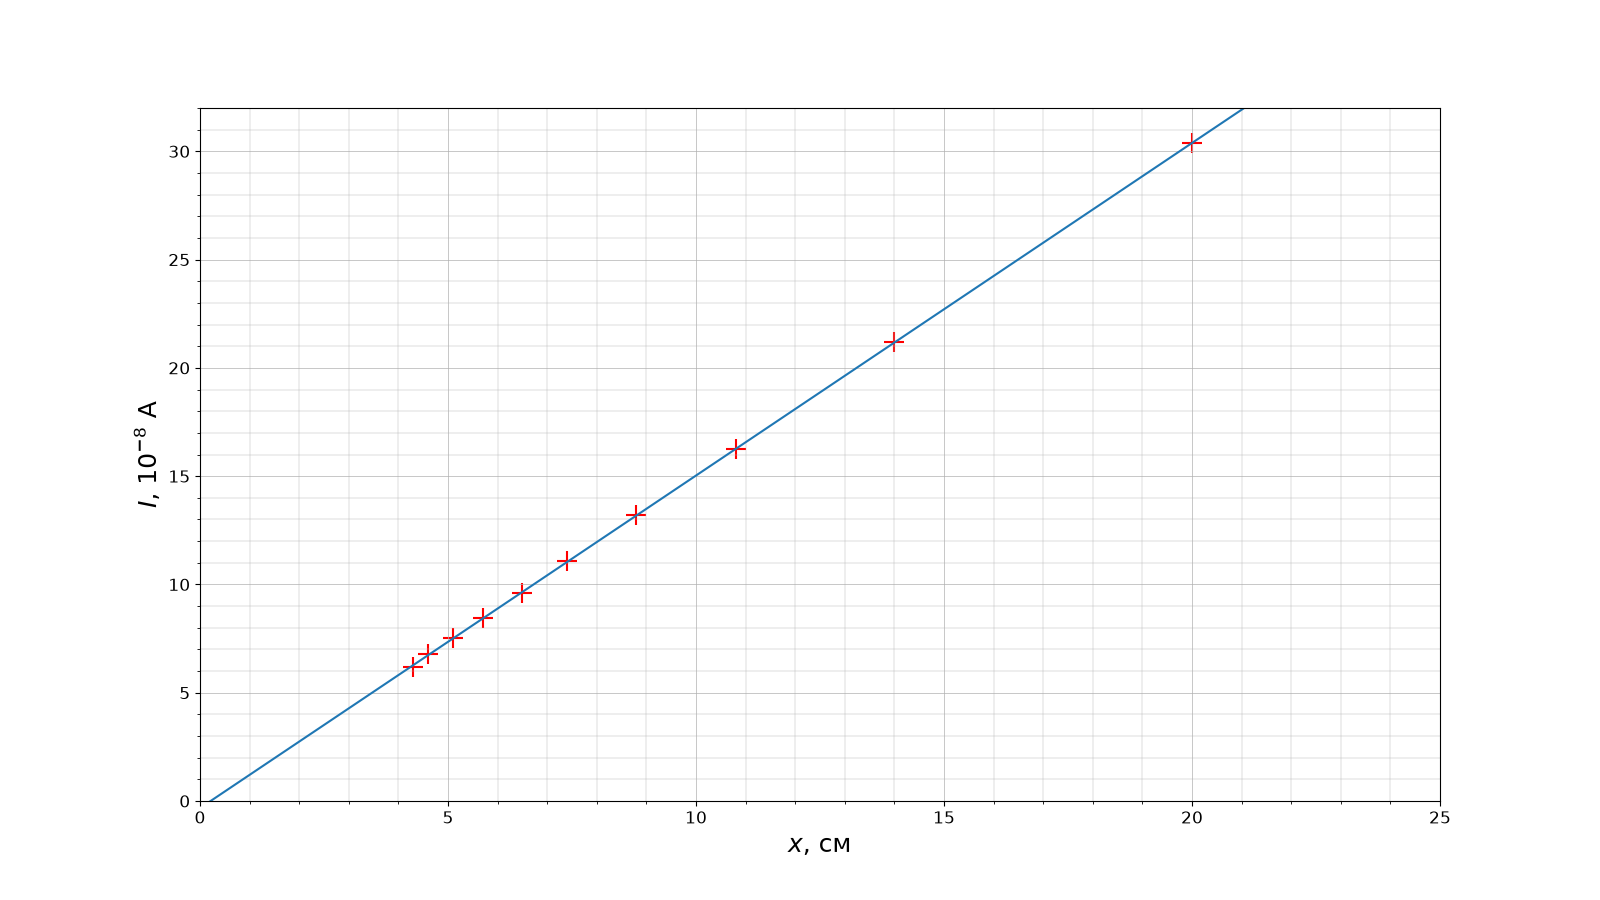
\includegraphics[scale=0.47]{p20.png}
	 	\caption{Зависимость $ I $ от $ x $}
	 \end{figure}

    \newpage
    
     Построим график зависимости тока $ I $ от отклонения зайчика $ x $. Аппроксимируем полученный результат МНК прямой $y=ax+b$.

    $a = 1.536 * 10^{-8}$ А/см

    $\sigma_a = 0.003*10^{-8}$ А/см

\noindent    По формуле (2) $C_I=(4.12 \pm 0.03) \frac{A}{\text{мм/м}}$
    
$
\frac{\sigma_{C_I}}{C_I}
=
\sqrt{
\left(\frac{\sigma_a}{a}\right)^2
+
\left(\frac{\sigma_{\tg\alpha}}{\tg\alpha}\right)^2
}
\approx 0.03
$

$S_I=\frac{1}{C_I}=0.24 \frac{\text{мм/м}}{A}$ 

\subsection{Критическое сопротивление}

Измерим 2 последовательных отклонения зайчика при разомкнутом контуре:
    
    $ x_n = 18,3$  см, $x_{n+1} = 14,0$ см 

\noindent Тогда мы получаем, что логарифмический декремент $ \Theta_0  = 0.27$

\noindent Период колебаний примерно равен $ T_0  = 3.3$ c

Теперь для расчёта $ \Theta $  проведём измерение отклонений зайчика после размыкания ключа $ П $, увеличивая $ R $ магазина от примерно $ 3R_{кр} $  до 1$ 0R_{кр} $. Подсчитаем при этом логарифмический декремент по формуле (3) и отношение для расчёта $ R_{кр} $ по формуле (4). Результаты сведем в таблицу 2:

\begin{table}[h]
	\centering
	\caption{Результаты измерений при свободных колебаниях}
	\begin{tabular}{|c|c|c|c|c|c|}
		\hline
		$ N $& $R$, кОм & $ x_n, $ см &$ x_{n+1}, $ см & $ \Theta $ & $ R_{кр} $, кОм\\
		\hline
		1 & 16.5 & 16.8 & 1.8 & 2.23 & 5.11\\
		2 & 19.3 & 14.4 & 2.2 & 1.88 & 5.10 \\
		3 & 22.0 & 12.7 & 2.4 & 1.67 & 5.20 \\
		4 & 24.8 & 11.3 & 2.5 & 1.51 & 5.33 \\
		5 & 27.5 & 10.2 & 2.6 & 1.37 & 5.39 \\
		6 & 30.3 & 9.3 & 2.6 & 1.27 & 5.51 \\
		7 & 33.0 & 8.5 & 2.6 & 1.18 & 5.60 \\
		8 & 38.5 & 7.3 & 2.6 & 1.03 & 5.72 \\
		9 & 44.0 & 6.4 & 2.7 & 0.86 & 5.44 \\
		10 & 49.5 & 5.7 & 2.6 & 0.78 & 5.56 \\
		11 & 55.0 & 5 & 2.3 & 0.78 & 6.24 \\
        % критическое сопротивление не считал!!!!! 
		\hline
	\end{tabular}% 
	\label{resR}% 
\end{table}% 

Видно, что все $R_\text{кр}$ примерно равны, поэтому возьмём среднее:

$R_\text{кр} = (5.5 \pm 0.1)$ кОм

$\sigma_R = 0.1$ кОм


\newpage

Теперь соберем схему согласно рис.2. 

\begin{table}[h]
	\centering
	\caption{Результаты измерений при динамическом режиме}
	\begin{tabular}{|c|c|c|c|}
		\hline
	$ N $ & $ R, $ кОм & $ x_{max}$, см \\
		\hline
		1 & 50 & 21.5 \\
		2 & 40 & 20.4 \\
		3 & 30 & 19.2 \\
		4 & 20 & 17.6 \\
		5 & 10 & 14.6 \\
		6 & 2 & 7.2  \\
		\hline
	\end{tabular}% 
	\label{resL}% 
\end{table}% 

\begin{figure}[h]
	 	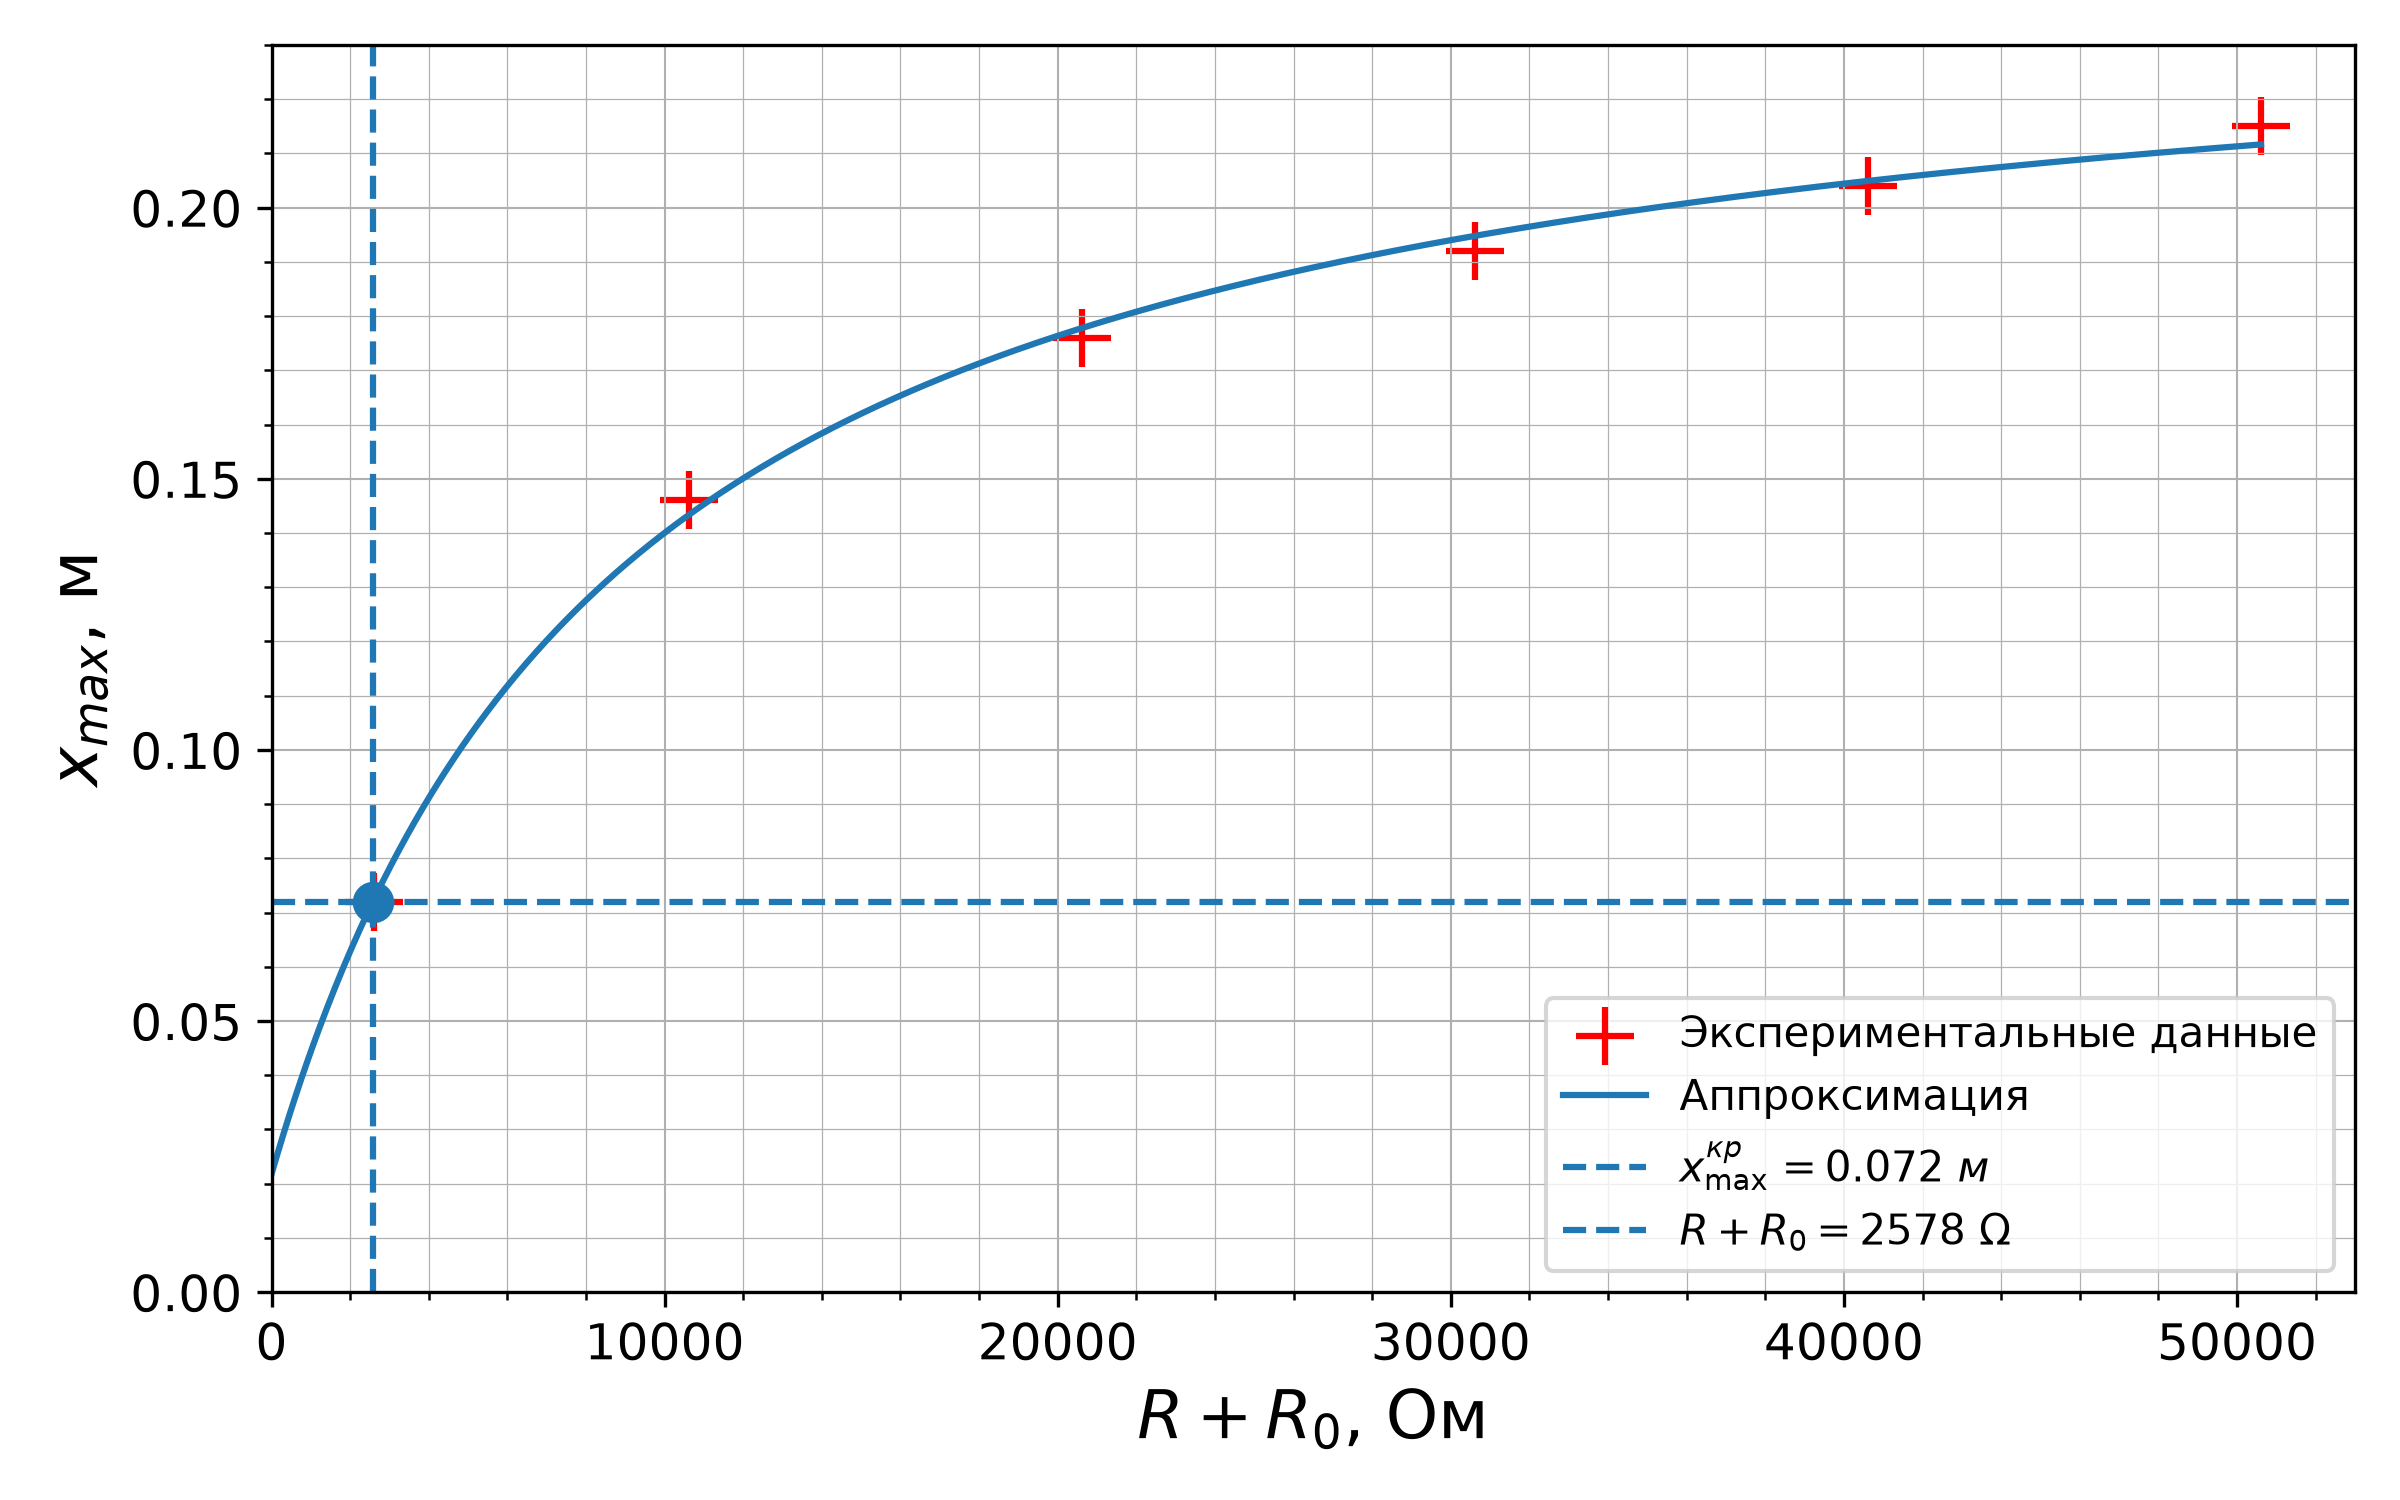
\includegraphics[scale=0.9]{p23.png}
	 	\caption{Зависимость $ x_{max} $ от $ R+R_0 $}
	 \end{figure}

Для определения критического сопротивления построим график зависимости
максимального отклонения зайчика $x_{\max}$ от суммарного сопротивления
цепи $R+R_0$. По экспериментальным данным построим аппроксимирующую
кривую.

При разомкнутом контуре было получено максимальное отклонение
\[
x_0 = 18{,}3\ \text{см},
\]
а логарифмический декремент затухания составил
\[
\Theta_0 = 0{,}27.
\]

Согласно поправке, максимальное отклонение гальванометра в режиме
свободных колебаний без учёта внутреннего затухания определяется
выражением
\[
x_{\max}^{\mathrm{св}}
=
x_0 e^{\Theta_0/4}.
\]

Подставляя экспериментальные значения, получаем
\[
x_{\max}^{\mathrm{св}}
=
18{,}3\,e^{0{,}27/4}
\approx
19{,}58\ \text{см}.
\]

Согласно соотношению, при критическом затухании максимальное
отклонение в $e$ раз меньше отклонения в режиме свободных колебаний:
\[
x_{\max}^{\mathrm{кр}}
=
\frac{x_{\max}^{\mathrm{св}}}{e}.
\]

Таким образом,
\[
x_{\max}^{\mathrm{кр}}
=
\frac{19{,}58}{e}
\approx
7{,}20\ \text{см}.
\]

Следовательно, на построенном графике необходимо найти точку
пересечения аппроксимирующей кривой с горизонтальной линией
\[
x_{\max}=7{,}20\ \text{см}.
\]

Из графика получаем для суммарного сопротивления
\[
R+R_0 \approx 2{,}58\ \text{кОм}.
\]

Учитывая, что внутреннее сопротивление гальванометра равно
\[
R_0=610\ \Omega=0{,}610\ \text{кОм},
\]
получаем критическое сопротивление внешней цепи:
\[
R_{\mathrm{кр}}
=
(R+R_0)_{\mathrm{кр}}-R_0.
\]

Подставляя значения, имеем
\[
R_{\mathrm{кр}}
=
2{,}58-0{,}610
\approx
1{,}97\ \text{кОм}.
\]

Окончательно:
\[
\boxed{R_{\mathrm{кр}}\approx1{,}97\ \text{кОм}}.
\]

\textbf{Сравнение результатов}

В работе были получены три значения критического сопротивления:
\[
R_{\mathrm{кр}}^{\mathrm{эксп}} = 5{,}5\ \text{кОм},
\]
полученное экспериментальным подбором, значение для стационарного
режима из п. 22
\[
R_{\mathrm{кр}}^{\mathrm{ст}} = 5{,}47\ \text{кОм},
\]
и значение для баллистического режима, определённое по графику в п. 23:
\[
R_{\mathrm{кр}}^{\mathrm{бал}} = 1{,}97\ \text{кОм}.
\]

Сравним полученные значения. Для стационарного режима относительное
расхождение с экспериментальным значением составляет
\[
\varepsilon_{\mathrm{ст}}
=
\frac{\left|R_{\mathrm{кр}}^{\mathrm{ст}}
-R_{\mathrm{кр}}^{\mathrm{эксп}}\right|}
{R_{\mathrm{кр}}^{\mathrm{эксп}}}
\cdot 100\%
\approx
0{,}55\%.
\]

Для баллистического режима:
\[
\varepsilon_{\mathrm{бал}}
=
\frac{\left|R_{\mathrm{кр}}^{\mathrm{бал}}
-R_{\mathrm{кр}}^{\mathrm{эксп}}\right|}
{R_{\mathrm{кр}}^{\mathrm{эксп}}}
\cdot 100\%
\approx
64{,}2\%.
\]

Таким образом, значение критического сопротивления, полученное в
стационарном режиме, хорошо согласуется с экспериментальным значением,
тогда как результат, полученный в баллистическом режиме, значительно
от него отличается.


\subsection{Баллистическая постоянная}

Емкость конденсатора $ C = 2  $ мкФ. Установив делитель на положение 1/40.  

Теперь найдем баллистическую постоянную  по формуле:

\[
C_q^{\mathrm{кр}}
=
\frac{q}{\varphi_{\max}^{\mathrm{кр}}}
=
2a\frac{R_1}{R_2}
\frac{CU_0}{x_{\max}^{\mathrm{кр}}} = 2.61 \cdot 10^{-6} \text{Кл}
\]

Подсчитав погрешность по формуле 

\[
\sigma_{C_q^{\mathrm{кр}}}
=
C_q^{\mathrm{кр}}
\sqrt{
\left(\frac{\sigma_{U_0}}{U_0}\right)^2
+
\left(\frac{\sigma_a}{a}\right)^2
+
\left(\frac{\sigma_{x_{max}}}{x_{max}}\right)^2
}
=
0{,}06\cdot10^{-6}\ \text{Кл}
\]

\subsection{Сравнение периода свободных колебаний и время релаксации}

Подсчитаем время релаксации и сравним с периодом свободных колебаний:
\[
\tau = R_0 C \approx 1{,}1\ \text{мс}
\qquad\Rightarrow\qquad
\frac{T}{\tau}\approx 2{,}9\cdot10^3.
\]

\subsection{Вывод}

Итак, в этой работе мы изучили работу гальванометра в трех режимах: стационарном, свободных колебаний и баллистическом. Мы измерили критическое сопротивление контура $ R_{кр} $ тремя способами, а также нашли динамическую и баллистическую постоянную установки. 

\end{document}